%
\section{Design \& Architecture}\label{sec:design_architecture}
%
This chapter will explain about the scanner architecture, things that have considered while designing the component and some of the useful techniques I have analyzed to make an efficient scanner to extract \acs{OSS} component.

\subsection{Scanner Architecture}
 The first task of developing this scanner is creating an automated \acs{OSS} component extractor because manual extraction of \acs{OSS} component is a tedious and redundant task, finding an automated system will reduce the time consumption and make it more cost effective. The manual \acs{OSS} extraction is suitable for small projects with less \acs{OSS} components consumption which is a very rare case. The \acs{OSS} scanner is built as a web application in this project by considering some useful advantages like accessibility across the devices, less maintenance and increased flexibility and scalability. Like traditional web-application the \acs{OSS} scanner has front-end and back-end applications. I have decided to break down the \acs{OSS} scanner into three major parts which are \acs{OSS} component Analyzer, Evaluator and Reporter. 
 \begin{figure}[h!]
 	\includegraphics[width=15cm]{includes/architetcure.png}
 	\centering
 	\caption{\acs{OSS} scanner architecture}
 	\label{fig:architecture}
 \end{figure}
\newpage
The figure ~\ref{fig:architecture} shows where the three major parts have been placed in the web -application. The \acs{OSS} component analyzer will be developed in the front-end because as per the research question the \acs{OSS} components should be scanned in the front-end(web browser). Once the \acs{OSS} components are extracted from the project, the meta information(name and version) will be sent to the \acs{OSS} component evaluator for finding the vulnerabilities. The OSS component evaluator and reporter are developed in the back-end. To make a clear understating, the figure ~\ref{fig:sequence} will show clear interaction between the components.
\begin{figure}[h!]
	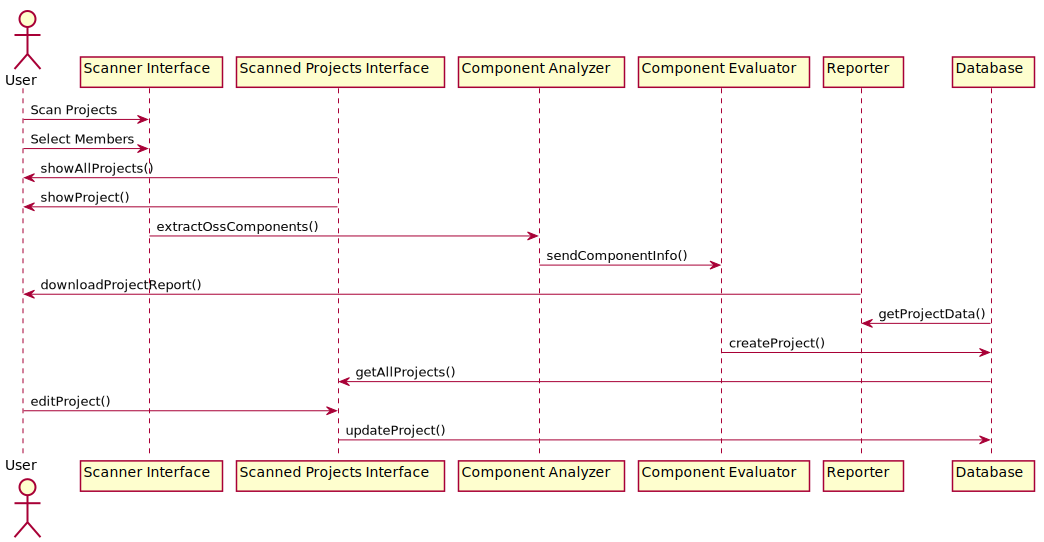
\includegraphics[width=15cm]{includes/sequence_diagram.png}
	\centering
	\caption{\acs{OSS} scanner sequence diagram}
	\label{fig:sequence}
\end{figure} 
\subsection{Scanner Components}

As shown in figure ~\ref{fig:architecture} there are three main components involved in the design and architecture of the \acs{OSS} scanner. Following are the components which are inter related to each other and gives a big picture of their functionality. \acs{OSS} Component Analyzer, \acs{OSS} Component Evaluator and \acs{OSS} Reporter.
\begin{description}
	\item [$\bullet$ OSS Component Analyzer:] This component is mainly responsible for extracting the \acs{OSS} components used in the projects. This particular task should be performed on the client side where the scanning should take place in the browser. The inputs required in this interface by the user are Project name, description, members and project directory. After receiving the inputs, there are two stages of the automation process, first the scanner will detect what type of application framework is given as input so that the scanner can parse the targeted file for the further process. Once the target file is parsed, the second process will extract the \acs{OSS} component name and the version used in the project. It creates \acs{JSON} data with basic project information along with the list of \acs{OSS} components and its version. Overall the primary goal of this component is to extract all the \acs{OSS} components and It will send the data evaluation process.
	
	\item [$\bullet$ OSS Component Evaluator:] This component evaluates the \acs{OSS} components which are extracted by the analyzer. The evaluation process component will be developed as a back-end application so that the process will be performed on the server side. This evaluation is performed with the help of \acs{NVD} database \acs{API} service. The extracted \acs{OSS} components will be searched in the \acs{NVD} database by using its name and version to find the known vulnerabilities registered under the respective component version. This component will be running asynchronously in the server because a project can have n-number of \acs{OSS} components. Once the \acs{OSS} components are evaluated, the information which is collected from the \acs{NVD} database is used for analysing the risk level of each \acs{OSS} component. Finally all the information is converted as a \acs{JSON} file and stored as container in Azure data storage.
	
	\item [$\bullet$ OSS Reporter:] This component is a part of the scanner’s user interface where the user can download the \acs{OSS} report of the project. This report shows all the basic information of the project and its \acs{OSS} component along with the vulnerability and the risk level of each component. This component simply generates a pdf report with all the above information retrieved from the database.
	
\end{description}
\subsection{Design Challenge}
Almost every software product development project has a unique set of problems. These issues can be a roadblock to development throughout system design and, more importantly, during implementation. There were several difficulties faced throughout the implementation of this thesis. The major problems that need to be addressed and a solution formed are listed below.
\begin{description}
	\item [$\bullet$ Application framework:] Because I had never worked with Angular framework before, the first hurdle I had while starting implementation was familiarizing myself with it. I got acquainted to the Angular environment with the aid of several online tutorials and hands-on programming.
	
	\item [$\bullet$ File structure:] The next challenge for me was trying to create a generic function that can extract the \acs{OSS} component name version from respected config files of the software project. This challenge was pretty time consuming because each software project can be built by using a different application framework and also each application framework has its own dependency manager. For instance, the Ruby on Rails application framework uses RubyGems as a dependency manager and it generates a file called Gemfile where all the \acs{OSS} components used in the projects are registered. Likewise Django has requirements.txt file, Dotnet has packages.config file, etc.
	
	
	\item [$\bullet$ Finding the right regex:] Another challenge was finding the right regex for each config file. The harder part was extracting the \acs{OSS} component names and version from config files like Gemfile and requirements.txt but other config files are comparatively easy to parse and extract the information because most of the files are generated as either \acs{JSON} or \acs{XML} files.
	
	\item [$\bullet$ Verification:] Another issue was determining whether what I built corresponded to what was actually happening within the software. To do so, I ran my code on a set of test inputs whose results were already known and checked if my program produced the same results.
\end{description}
%
